\let\negmedspace\undefined
\let\negthickspace\undefined
\documentclass[journal]{IEEEtran}
\usepackage[a5paper, margin=10mm, onecolumn]{geometry}
\usepackage{tfrupee} 
\usepackage{gvv-book}
\usepackage{gvv}
\usepackage{cite}
\usepackage{amsmath,amssymb,amsfonts,amsthm}
\usepackage{algorithmic}
\usepackage{graphicx}
\usepackage{textcomp}
\usepackage{xcolor}
\usepackage{txfonts}
\usepackage{listings}
\usepackage{enumitem}
\usepackage{mathtools}
\usepackage{gensymb}
\usepackage{comment}
\usepackage[breaklinks=true]{hyperref}
\usepackage{tkz-euclide} 
\usepackage{listings}  
\usepackage{multirow}
\usepackage{hhline}    
\usepackage{multicol}                                       
\usepackage{lscape}
\begin{document}

\bibliographystyle{IEEEtran}
\title{11.16.2.2.2}
\author{EE24BTECH11011-Pranay Kumar}
\maketitle
\textbf{Question:} A die is thrown. Describe the following events:
\begin{itemize}
\item (i) AA: A number less than 7.
\item (ii) BB: A number greater than 7.
\end{itemize}
Also, find the following $A\cup B$ ,$A \cap B$

\textbf{Solution:}
\begin{enumerate}
\item \textbf{Total Number of Possible Outcomes:}
The sample space of rolling a fair six-sided die is:
\begin{align}
S = {1, 2, 3, 4, 5, 6}
\end{align}
This means there are 6 possible outcomes when a die is rolled.
\item \textbf{Probability of Events:}
\begin{align}
    P(A) &= P(X < 7) = 1 \quad \text{(since all outcomes are less than 7)} \\
    P(B) &= P(X > 7) = 0 \quad \text{(since no outcomes are greater than 7)}
\end{align}
Here, event \( A \) is a certain event because it includes all possible outcomes of the die roll. Event \( B \) is an impossible event since there are no outcomes greater than 6 on a standard die.
\subsection*{Boolean Algebra Derivations:}
The Boolean algebra derivations provided are:

\begin{align}
A + A' &= 1 \quad \text{(Law of Complementarity)}, \\
AB + A'B &= B \quad \text{(Distributive Law)}, \\
\implies P(AB) + P(A'B) &= P(B) \quad \text{(Probability of the above)}, \\
B + B' &= 1 \quad \text{(Law of Complementarity)}, \\
AB + AB' &= A \quad \text{(Distributive Law)}, \\
\implies P(AB) + P(AB') &= P(A) \quad \text{(Probability of the above)}, \\
A + B &= AB + AB' + A'B \quad \text{(Expansion of Union)}, \\
\implies P(A + B) &= P(AB) + P(AB') + P(A'B) \quad \text{(Probability of the above)}.
\end{align}


\subsection*{Step 1: Find \( A \cup B \) (Union of \( A \) and \( B \))}
Using the expansion of the union:
\[
A + B = AB + AB' + A'B
\]
Taking probabilities on both sides:
\[
P(A + B) = P(AB) + P(AB') + P(A'B)
\]

From the problem:
\[
P(A) = 1, \quad P(B) = 0, \quad \text{and} \quad P(AB) = 0 \quad \text{(since \( A \) and \( B \) are mutually exclusive)}.
\]
\[
P(AB') = P(A) - P(AB) = 1 - 0 = 1,
\]
\[
P(A'B) = P(B) - P(AB) = 0 - 0 = 0.
\]

Substituting these values:
\[
P(A + B) = 0 + 1 + 0 = 1
\]

Thus:
\[
A \cup B = 1
\]

\subsection*{Step 2: Find \( A \cap B \) (Intersection of \( A \) and \( B \))}
The intersection \( A \cap B \) is the event where both \( A \) and \( B \) occur simultaneously. From the problem:
\[
A: \text{A number less than 7}, \quad B: \text{A number greater than 7}.
\]

Since no number can be both less than 7 and greater than 7 at the same time, \( A \cap B \) is an impossible event. Therefore:
\[
P(AB) = 0
\]

Thus:
\[
A \cap B = 0
\]

\subsection*{Final Results:}
\[
A \cup B = 1 \quad \text{(The union of \( A \) and \( B \) is certain because \( A \) is certain)},
\]
\[
A \cap B = 0 \quad \text{(The intersection of \( A \) and \( B \) is impossible because \( A \) and \( B \) are mutually exclusive)}.
\]


\item \textbf{Probability Mass Function (PMF):}
\begin{align}
    P_X(x) = \begin{cases}
        \frac{1}{6}, & x \in \{1,2,3,4,5,6\} \\
        0, & \text{otherwise}
    \end{cases}
\end{align}
The PMF describes the probability distribution of the outcomes of the die roll. Each outcome from 1 to 6 has an equal probability of \( \frac{1}{6} \).

\item \textbf{Cumulative Distribution Function (CDF):}
\begin{align}
    F_X(k) = \begin{cases}
        0, & k < 1 \\
        \frac{k}{6}, & 1 \leq k \leq 6 \\
        1, & k > 6
    \end{cases}
\end{align}
The CDF gives the probability that the die roll will result in a value less than or equal to \( k \). It increases linearly from 0 to 1 as \( k \) increases from 1 to 6.

\item \textbf{Monte Carlo Simulation:}
We approximate probabilities by simulating a large number of die rolls and computing relative frequencies. This method is useful for verifying theoretical probabilities and understanding the behavior of random variables through empirical data.

\item \textbf{Additional Insights:}
\begin{itemize}
    \item The events \( A \) and \( B \) are mutually exclusive because they cannot occur simultaneously. This is evident from the fact that \( P(AB) = 0 \).
    \item The probability of the union of two mutually exclusive events is the sum of their individual probabilities, as shown by \( P(A + B) = P(A) + P(B) \).
    \item The PMF and CDF are fundamental tools in probability theory for describing the distribution of discrete random variables.
\end{itemize}
\begin{figure}[H]
    \centering
    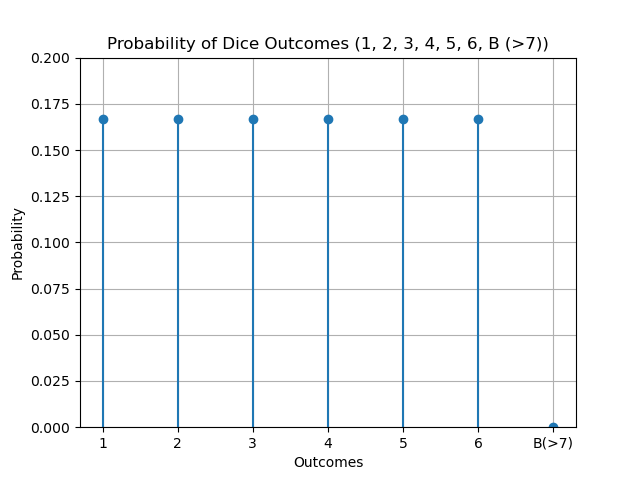
\includegraphics[width=\columnwidth]{figs/fig.png}
    
    \label{fig:pmf}
\end{figure}

\end{enumerate}
\end{document}

